\section{Observability Layer}
\begin{frame}
    \frametitle{ Components}
    \begin{figure}
        \centering
        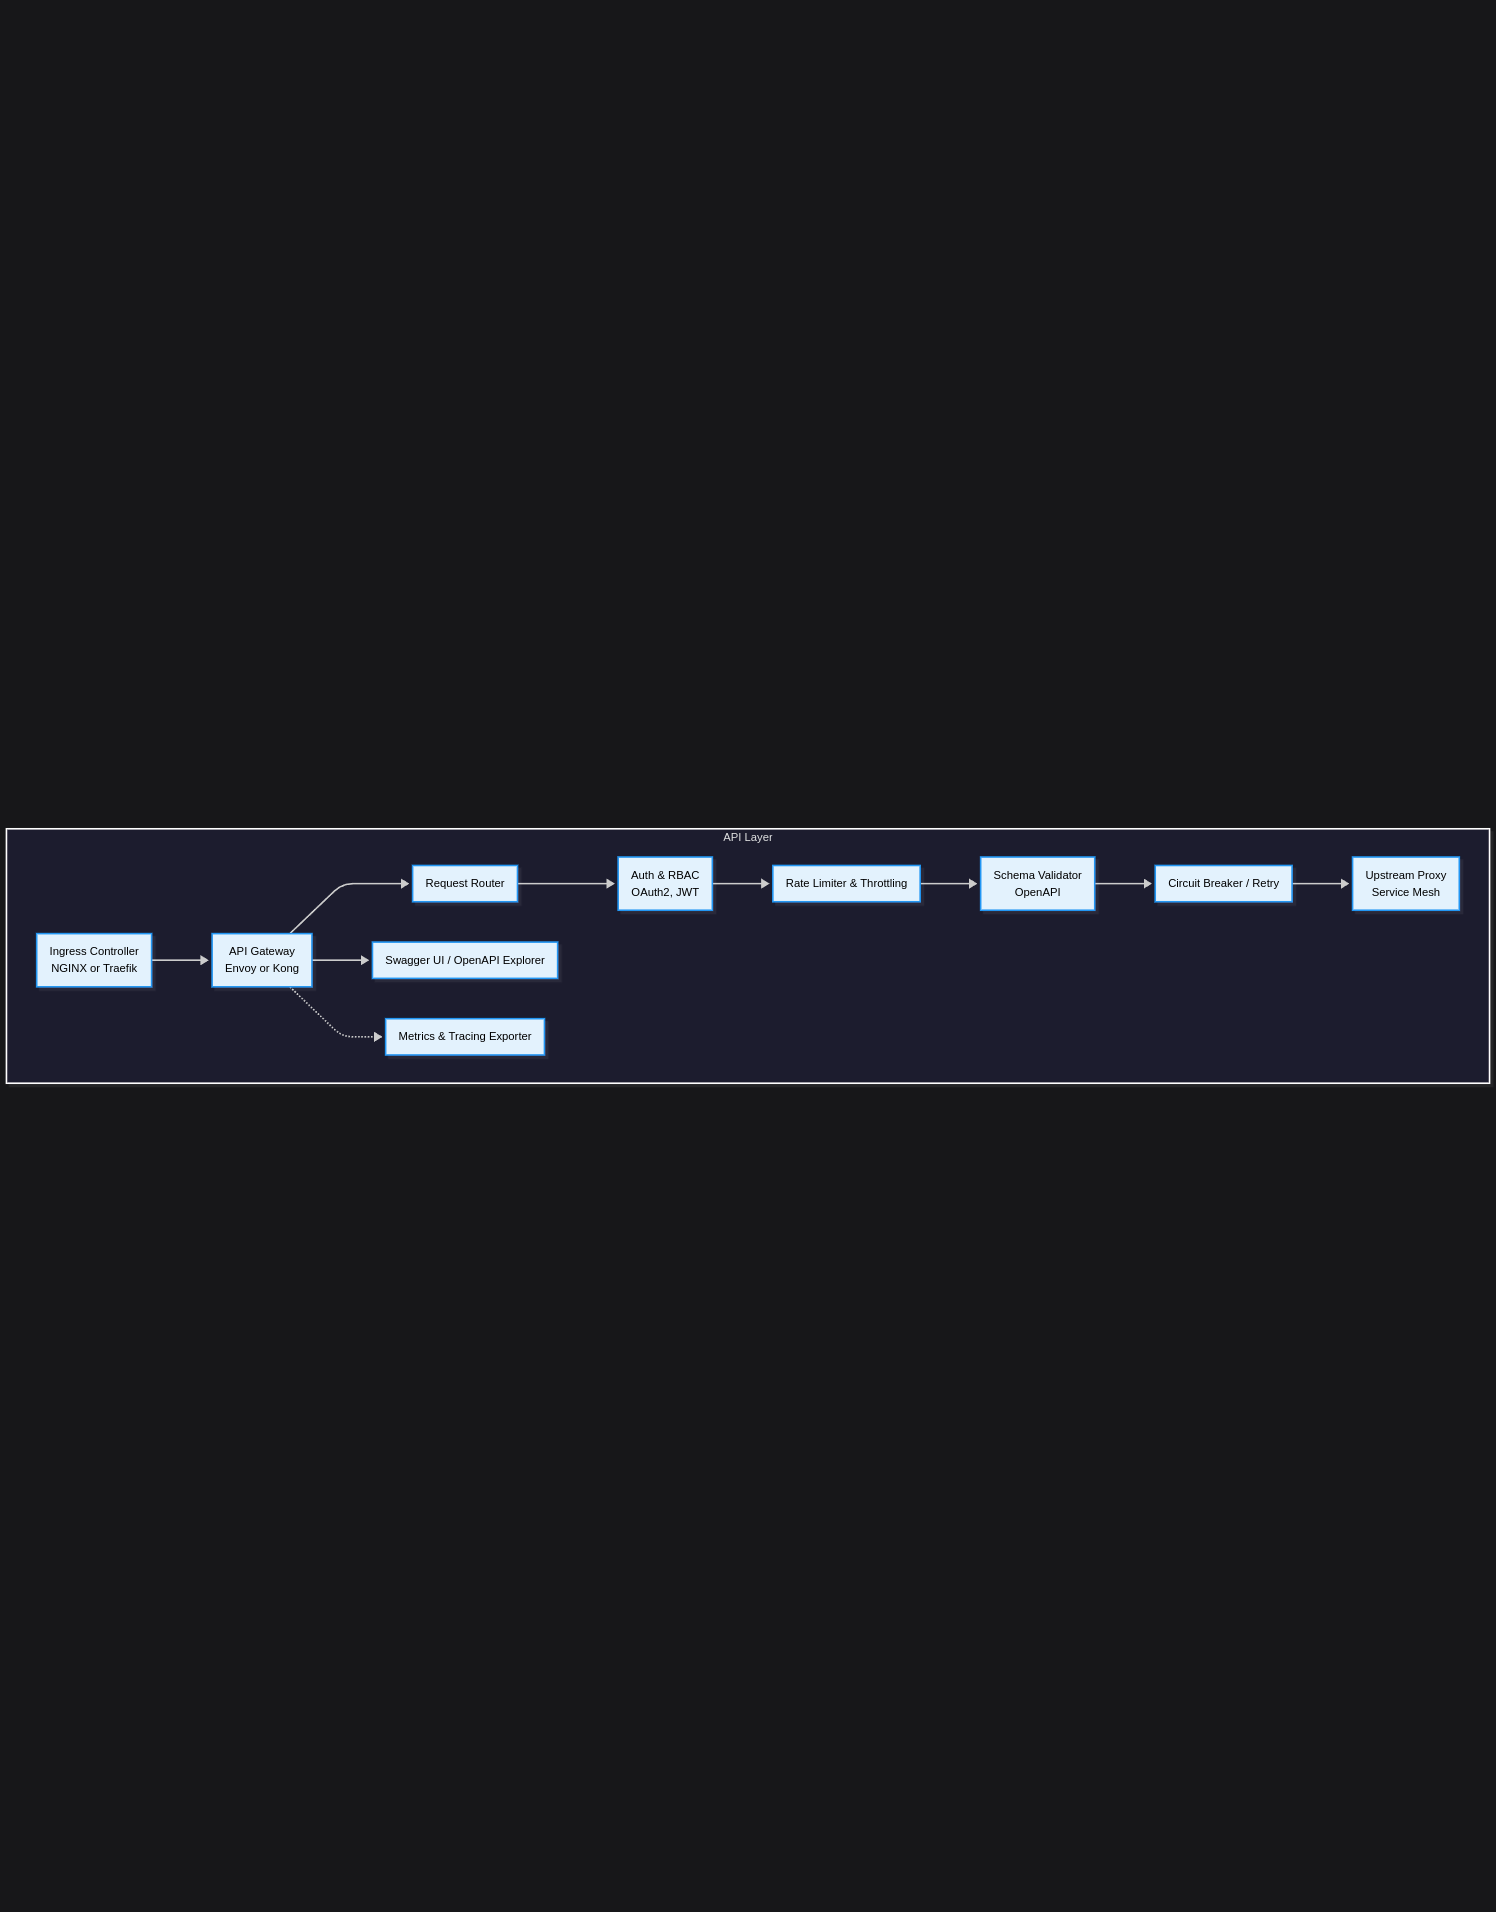
\includegraphics[width=0.8\textwidth]{obs/layout.png} % Adjusted the scale of the image to 0.5
        \caption{Layout}
    \end{figure}
\end{frame}

\begin{frame}
    \frametitle{Sequence Flow}
    \begin{figure}
        \centering
        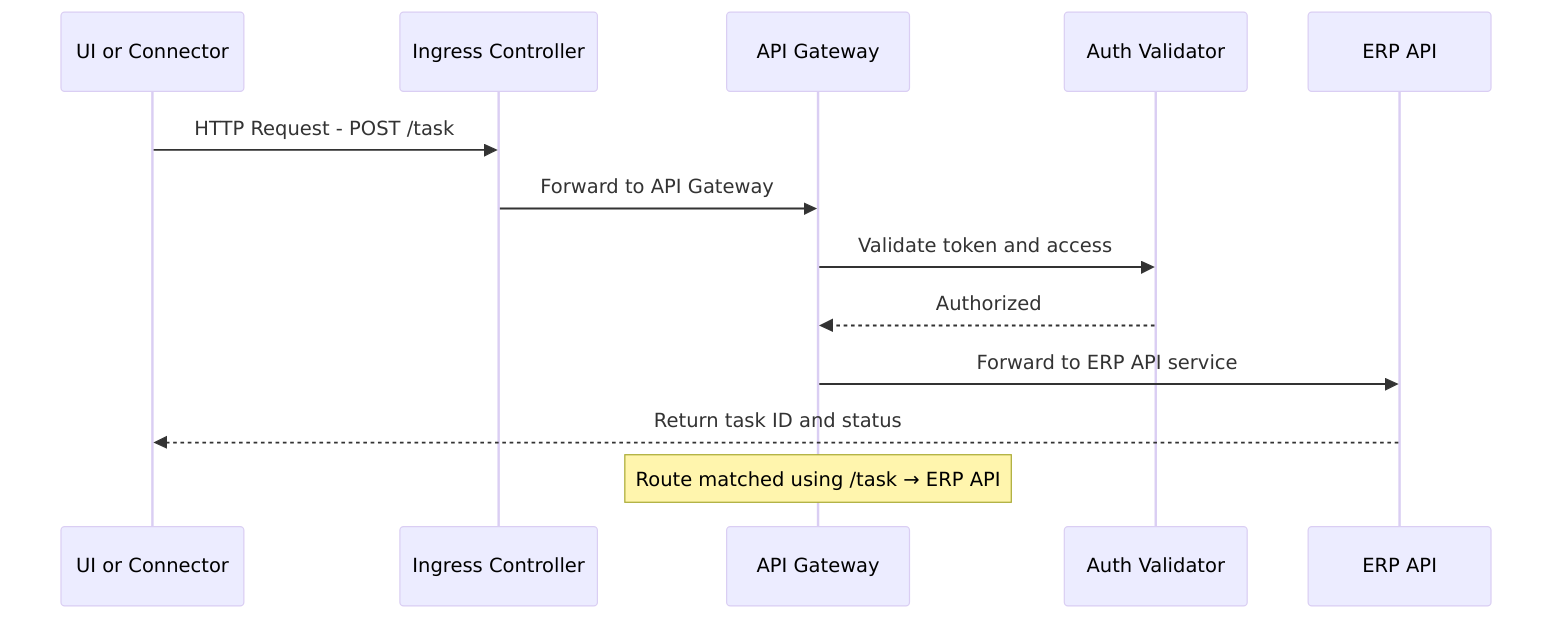
\includegraphics[width=0.8\textwidth]{obs/sequence.png} % Adjusted the scale of the image to 0.5
        \caption{Sequence Flow}
    \end{figure}
\end{frame}


\begin{frame}
    \frametitle{Components}
    \begin{itemize}
        \item \textbf{Prometheus}: Collect time-series metrics from ETL, agents, ERP, and infrastructure.
        \item \textbf{Grafana}: Visualize dashboards for system performance, agent status, SLA tracking.
        \item \textbf{Loki or ELK}: Aggregate logs from all services and containers for debugging and traceability.
        \item \textbf{Jaeger or Tempo}: Trace request paths across microservices for deep diagnostics.
        \item \textbf{Alertmanager}: Trigger alerts based on thresholds, time windows, or error patterns.
        \item \textbf{Audit Log DB}: Store agent actions, task transitions, and version history in a structured format.
        \item \textbf{Data Tagger}: Append project, task, and agent labels to each event for query and filtering.
    \end{itemize}
\end{frame}

% \begin{frame}
%     \frametitle{Technical Responsibilities}
%     \begin{table}[h!]
% \centering
% \renewcommand{\arraystretch}{1.2}
% \begin{tabular}{|p{3cm}|p{7cm}|}
% \hline
% \textbf{Component} & \textbf{Technical Responsibility} \\
% \hline
% Prometheus & Scrapes metrics from `/metrics` endpoints and stores time-series data \\
% \hline
% Grafana & Provides dashboards using Prometheus, Loki, and TimescaleDB data sources \\
% \hline
% Loki or ELK & Collect logs via Fluent Bit, Vector, or Beats and index for search \\
% \hline
% Jaeger or Tempo &
% Data Tagger & Append project, task, and agent labels to each event for query and filtering \\
% \hline
% \end{tabular}
% \caption{Observability Layer - Functional Responsibilities (Part 2)}
% \end{table}
% \end{frame}

% \begin{frame}
%     \frametitle{Technical Responsibilities}
%     \begin{table}[h!]
% \centering
% \renewcommand{\arraystretch}{1.2}
% \begin{tabular}{|p{3cm}|p{7cm}|}
% \hline
% \textbf{Component} & \textbf{Technical Responsibility} \\
% \hline
% Prometheus & Scrapes metrics from `/metrics` endpoints and stores time-series data \\
% \hline
% Grafana & Provides dashboards using Prometheus, Loki, and TimescaleDB data sources \\
% \hline
% Loki or ELK & Collect logs via Fluent Bit, Vector, or Beats and index for search \\
% \hline
% Jaeger or Tempo & Capture span-based traces for request analysis across ETL, API, agents \\
% \hline
% Alertmanager & Manage rules for alerts, notify via email, Slack, or webhook \\
% \hline
% Audit Log DB & TimescaleDB or Postgres schema storing agent events and task state history \\
% \hline
% Data Tagger & Inject labels (project, agent, doc version) into metrics, logs, and traces \\
% \hline
% \end{tabular}
% \caption{Observability Layer - Technical Responsibilities}
% \end{table}
% \end{frame}